\subsection{Problem characteristics}
Origami has been around for a long time. It originated in China and Japan and
spread all around the world\cite{wiki:history-of-origami}. Origami is
recognized as the art of paper folding.
Recently it is becoming increasingly popular in a scientific context.
Although known for centuries, it still exhibits properties that are useful
in many different contexts, e.g.
space exploration\cite{origami-in-orbit}, or deploying solar arrays\cite{solar-panel-origami}.
Mathematicians started recognizing material folding as a distinct
branch known as \hyperref[dictionary:computational-origami]{\textit{computational origami}}.
The field has seen a tremendous development in the past couple decades especially in the software space.
Although dynamic, there are still many open problems \cite{mit-open-problems}.
Beginners fold origami following step-by-step instructions.
More advanced origamists will use a \hyperref[dictionary:crease-pattern]{\textit{crease pattern}}
to form a \hyperref[dictionary:folded-state]{\textit{folded state}}.
The process of origami creation consists of two stages: \textit{design} and \textit{folding}.

\begin{figure}[H]
\caption{A crease pattern for the popular origami crane model}
  \centering
    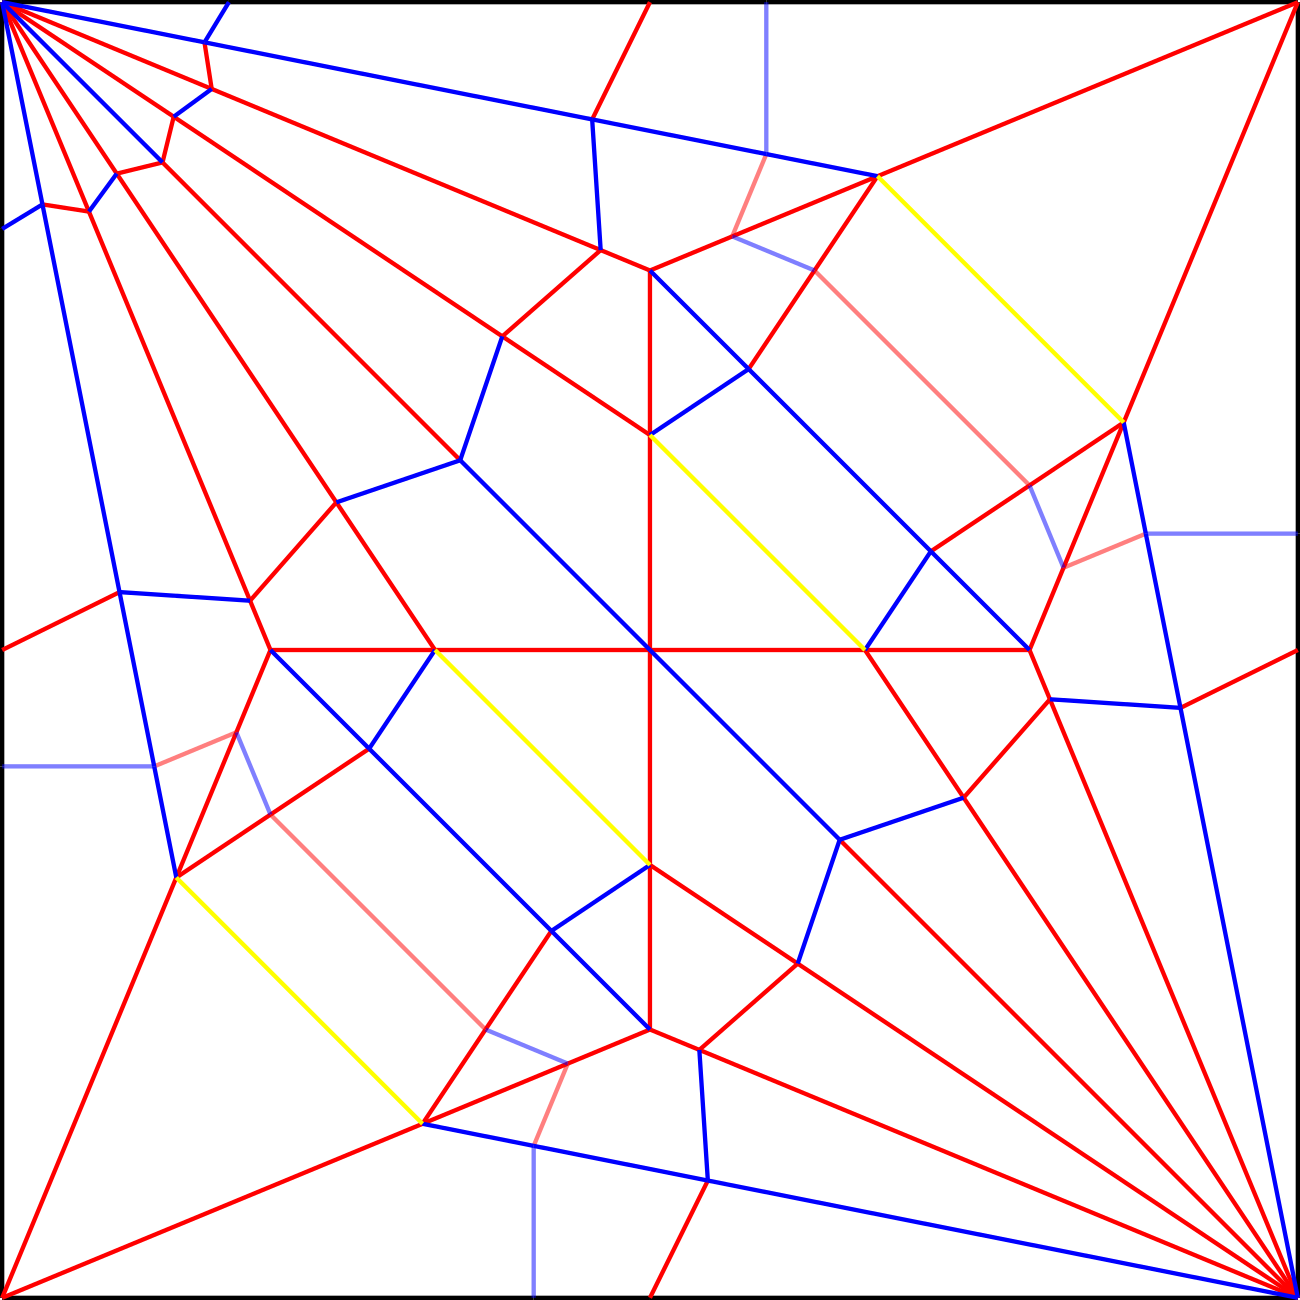
\includegraphics[width=0.8\textwidth]{assets/crane-crease-pattern.png}
\end{figure}

\subsection{Motivation}

Even though origami seems to be a child's play, at times
people would get discouraged whilst following the origami instructions due to
the lack of details they expose.

We would like to provide a way for beginners (and advanced origamists alike) to visualize step-by-step the folding process of the origami pattern that they provide.
While there exist some programs aiding the process of design, there is no satisfactory solution
that would present the process of folding as it would be carried out manually.

We have evaluated existing solutions, and the one that resembles 
what we would like to achieve the most \cite{origami-simulator} provides a way to load a crease pattern
and display the process of folding, however it does not allow to visualize the process step-by-step, it only allows 
to go from a flat sheet of paper to a folded state immediately. It also bypasses some physical properties, such as the fact that the
paper should collide with itself.


\begin{figure}[H]
\caption{Origami simulator by Amanda Ghassaei}
  \centering
    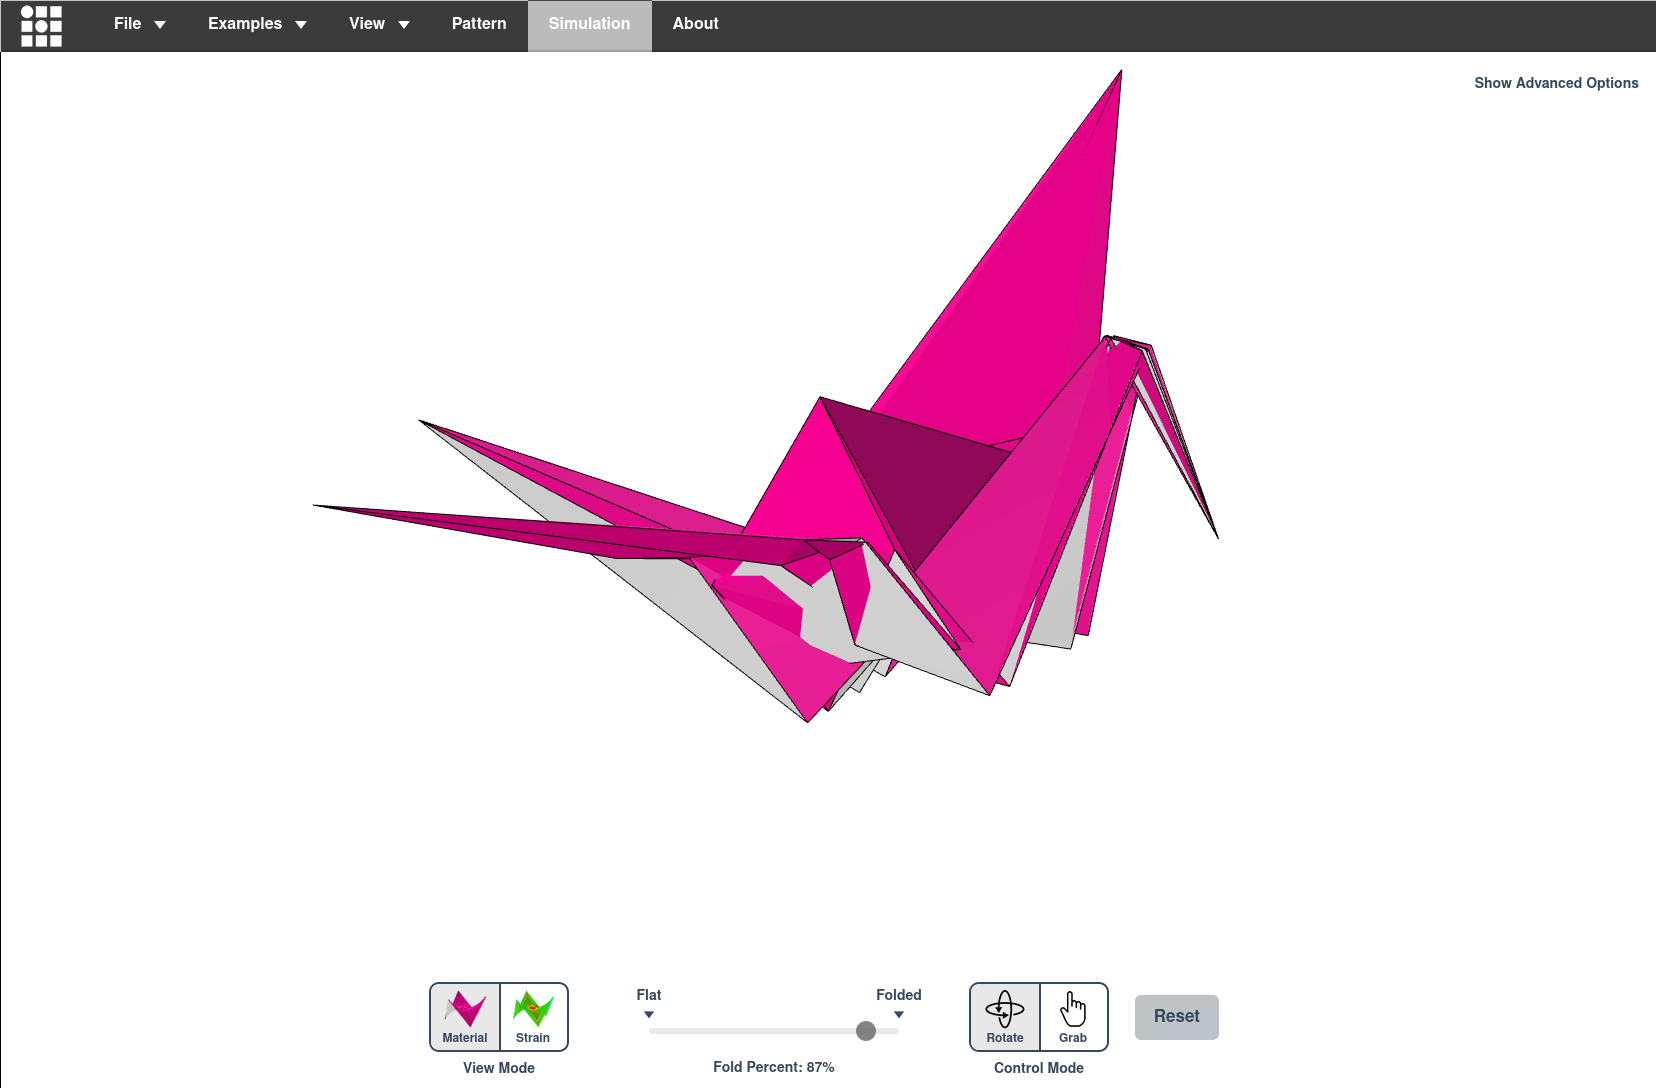
\includegraphics[width=0.8\textwidth]{assets/origami-simulator.png}
\end{figure}

\subsection{Product Vision}

\subsubsection{Functionality}

Our main goal is to create a platform to visualize the origami model in 3D,
in every step of the folding process, while animating the transitions between the steps.

The inseparable component of the system would be a file format describing the folding steps necessary to complete the origami.\\

\noindent \textbf{The users would be able to:}
\begin{itemize}
	\item load the folding instruction
	\item choose the step of the instruction that they want to visualize
	\item rotate the scene
    \item zoom in and out
	\item move around the scene
	\item pause the animation at any time, and move back and forth
\end{itemize}

\subsubsection{Technology}

Our application will consist of two layers - backend and frontend.

Backend part will serve frontend pages, and be responsible
for storing user files.

Frontend part will handle user interaction, computations on the origami model,
3D visualizations, and communication with backend.

We have decided to use well-known and tested technologies.
For the backend part, we are going to use \tech{Go} language,
using standard library to write the server part.

For the frontend, we will use vanilla \tech{JavaScript}
for user interface and computations,
and we will perform 3D rendering using \tech{Three.js} library
that is built on top of \tech{WebGL}.

\begin{figure}[H]
	\caption{Technology stack}
	\centering
	\begin{tikzpicture}
	\node (backend) at (0,0) [draw,thick,minimum width=4cm,label=north west:Backend] {
		
\includegraphics[width=.25\textwidth]{assets/go-logo-blue.png}
	};
	\node[below = of backend] (frontend) [draw,thick,minimum width=4cm, label=north west:Frontend] {
		
\includegraphics[width=.15\textwidth]{assets/javascript-logo.png}
		
\includegraphics[width=.30\textwidth]{assets/three-js-logo.png}
	};
	\draw[<->,thick] (backend.south) -- (frontend.north);
	\end{tikzpicture}
\end{figure}


\subsection{Feasibility Study}

Both \tech{Go} and \tech{JavaScript} are widely spread and actively maintained languages.
There is a strong community surrounding both of them.
\tech{Three.js} is the most popular library for 3D \tech{WebGL} rendering.

Therefore, we are not expecting problems connected with the tools we have selected.

Since the project will require a lot of knowledge from the computational origami
field, we will have to research the existing materials on this topic.
The most promising resource seems to be a MIT course by
Eric Demaine \cite{mit-course}, and a book co-authored by the same person -
Geometric Folding Algorithms\cite{origami-book}.
Various papers are also available which might come in handy, especially those regarding software implementations.


\subsection{Threat Assessment}

Playing with the intersection between reality and computer science has always
been a challenging task.
Here, we are trying to tackle a problem that has not been discussed previously.
Every year the field of computational origami sees a progress,
so the mathematics behind it are not yet well developed.
We foresee many challenges along the way, such as:

\begin{itemize}
	\item NP-hardness - some problems that we will face are in general proved to be NP-hard.
		Example of such a problem can be computing layer ordering based on a crease pattern.
		We will have to overcome them either using approximate methods, or coming up with solutions that will avoid them.

	\item physical properties of a paper - if we would like to support complex physical properties,
		there is a lot of features that would require a separate set of computations simulating paper physics, e.g.
		\begin{itemize}
			\item inflating
			\item curving 
			\item cutting
		\end{itemize}

	\item performance - web browser are still not well optimized to carry out 3D computations and render 3D graphics in real time.
		The system will have to be highly optimized, in order to be usable.
		State of the art programs offload computational payload to GPU.

	\item mathematics - we don't have a lot of experience in writing complex simulations utilizing complicated mathematical formulas.
		Even computing a simple paper fold requires physical computations such as computing strain on different parts of the paper.

	\item 3D graphics - we have some experience working with 3D, however only from the user perspective.
		We have little experience in creating 3D graphical software.

\end{itemize}

That all being said, we believe we are able to undertake this problem and provide a solution to it.
While challenging it is also rewarding in terms of business value and as a unique product in the field.


\subsection{Dictionary} \label{dictionary}

\begin{description}
	\item[computational origami] \label{dictionary:computational-origami} -- a recent branch of computer science studying efficient algorithms for solving paper-folding problems.\cite{recent-results-in-computational-origami:paper}
	\item[crease] -- a line segment, along which a sheet of paper folds.
	\item[crease pattern] \label{dictionary:crease-pattern} -- a pattern of lines formed by creases that is created after unfolding the origami flat. For an example see figure \ref{fig:creasepattern}.
	\item[folded state] \label{dictionary:folded-state} -- An assembled origami model. Or alternatively, a sheet of paper folded along the crease pattern.
	\item[mountain] -- a fold of paper along the crease, such that the facets on the sides of the crease are facing downwards.
					\begin{figure}[H]
						\caption{Example of a mountain crease}
						\centering
						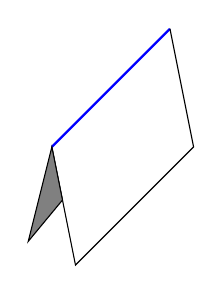
\begin{tikzpicture}[scale=1.5]
							\draw[blue, thick] (0,0) -- (1,1);
							\draw (1,1) -- (1.2, 0) --  (0.2, -1) -- (0,0);
							\filldraw[fill=gray] (0, 0) -- (-0.2, -0.8) -- (0.09, -0.45) -- cycle;
						\end{tikzpicture}
					\end{figure}
	\item[valley] -- A fold of paper along a crease, such that the facets on the sides of the crease are facing upwards.
					\begin{figure}[H]
						\caption{Example of a valley crease}
						\centering
						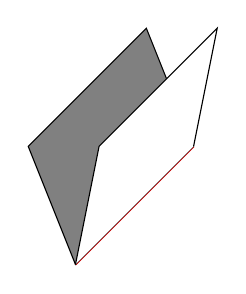
\begin{tikzpicture}[scale=1.5]
							\draw[red, thick] (0,0) -- (1,1);
							\filldraw[fill=gray] (0, 0) -- (-0.4, 1) -- (0.6, 2) -- (1, 1) -- cycle;
							\filldraw[fill=white] (1,1) -- (1.2, 2) --  (0.2, 1) -- (0,0);
						\end{tikzpicture}
					\end{figure}
	\item[mountain-valley assignment] -- an assignment of mountain or valley to the creases on the crease pattern.
	\item[.fold file] -- a file that conforms to the FOLD\cite{fold:paper} specification.
	\item[Instruction] -- a \textit{.fold} file created by a user, representing a sequence of steps required to
		fold a sheet of paper into a complete origami figure.
	\item[Transition] -- a folding animation played between two steps.
	\item[Guide] -- a set of all Transitions derived from an Instruction. Can be represented using a \textit{.fold} file.
	\item[Model] -- 3D representation of an origami figure. 
	\item[FPS] -- frames per second.
	\item[target angle] -- the supplement of the dihedral angle between the two neighbouring faces,
		towards which the faces should fold.
\end{description}



